\section{Results}
\label{sec:results}

% Generated by paper/scripts/make_main_tables.py.
\begin{table*}[t]
\centering
\caption{Held-out system endpoints.  Admission and Ranking determine the
localization route; adding Abstention leaves every selected query and box
bitwise unchanged.  Deltas and paired 95\% image-cluster intervals are relative
to the frozen base.}
\label{tab:headline}
\scriptsize
\setlength{\tabcolsep}{3.1pt}
\begin{tabular}{lrrrrrr}
\toprule
System & Test5$\uparrow$ & Strict FPR95$\downarrow$ & $\Delta$Test5 [CI] & FPR95 red. [CI] & Elig. recall$\uparrow$ & Elig. $n\downarrow$ \\
\midrule
Frozen base & 72.16 & 51.21 & -- & -- & -- & -- \\
Admission + Ranking & 74.24 & -- & +2.08 [1.83, 2.35] & -- & 99.69 & 69.5 \\
ARROW-U2 (+ Abstention) & 74.24 & 47.02 & +2.08 [1.83, 2.35] & 4.19 [2.46, 6.20] & 99.69 & 69.5 \\
\bottomrule
\end{tabular}
\vspace{2pt}
\parbox{0.98\textwidth}{\footnotesize Percentages except eligible-query
count.  Frozen-to-ARROW rows are cumulative system comparisons with additional
head supervision; equal-supervision owner claims use
Tab.~\ref{tab:interference}.  Validation decomposition and parameter/runtime
accounting are supplementary.}
\end{table*}


\subsection{ARROW improves both deployed endpoints}
\method improves Test5 Acc@0.5 by \ArrowTestGain\ points (95\% paired
image-cluster CI [\ArrowTestGainLo, \ArrowTestGainHi]) and lowers
Strict-TN2031 FPR95 by \ArrowStrictGain\ points (CI
[\ArrowStrictGainLo, \ArrowStrictGainHi]); see Tab.~\ref{tab:main}.
Rejection cannot explain the localization gain: learned Admission plus Ranking
and full \arrowv have bitwise-identical localization records by construction.

The cumulative mechanism rows explain complementarity rather than independent
additivity.  The unrestricted complete-expression ranker is almost identical
to the base.  A static Admission prior helps modestly, and learned Admission
creates the main localization gain by constraining the comparison domain.  Yet
canonicalizing only the ranking expression---with geometry and eligibility
fixed---drops Acc@0.5 by more than ten points and changes 37.85\% of top-1
queries.  Admission defines who may compete; the complete expression decides
which instance wins.

% Generated by paper/scripts/make_main_tables.py.
\begin{table*}[t]
\centering
\caption{Ownership evidence at two representation strengths.  On ARROW-U2,
isolation improves rejection with unchanged localization.  On the strong e5
trunk, Isolated reduces FPR95 by 4.070 points versus Native without
changing REC, but does not beat capacity-matched Shared-Wide.}
\label{tab:ownership}
\scriptsize
\setlength{\tabcolsep}{3.5pt}
\begin{tabular}{llrrrrr}
\toprule
Trunk & Design & Params (K) & MAC/query (K) & Grad. cosine (three seeds) & REC$\uparrow$ & Strict FPR95$\downarrow$ \\
\midrule
ARROW-U2 & Shared scalar & -- & -- & -0.19/-0.25/-0.28 & 74.30 & 50.11 \\
ARROW-U2 & Isolated & -- & -- & zero & 74.30 & 47.30 \\
Strong e5 & Native e5 & 0 & 0.0 & -- & 88.969 & 88.282 \\
Strong e5 & Shared-128 & 50.3 & 49.5 & -0.063/+0.008/-0.011 & 88.973 & 85.442 \\
Strong e5 & Shared-Wide & 100.4 & 99.4 & -0.018/+0.032/+0.012 & 88.979 & 83.686 \\
Strong e5 & Isolated & 100.4 & 98.8 & zero by design & 88.976 & 84.211 \\
\bottomrule
\end{tabular}
\vspace{2pt}
\parbox{0.98\textwidth}{\footnotesize ARROW-U2 REC is Test5; strong-e5 REC
is RefCOCO TestA+TestB micro. Learned rows report three-seed means; Native is
deterministic. Shared-Wide and Isolated match total capacity
(100,362 vs. 100,358 parameters); Shared-Wide also gives each task a wider
210-d representation. Separate task-specific Adam states and zero weight decay
are used in every learned arm. The e5 trunk is a retrospective checkpoint
replay; its ownership matrix was frozen prospectively.}
\end{table*}


\subsection{Ownership, not output count, resolves conflict}
Table~\ref{tab:ownership} isolates feature ownership from output separation.
The shared scalar has negative Admission/Rejection gradient cosine in every
seed ($-0.190$, $-0.252$, $-0.281$), with sign-conflict fractions around
0.53--0.56.  Merely attaching separate outputs to the same trainable feature
surface leaves calibration FPR95 essentially unchanged; this separate-head
control is calibration-only and has no held-out Strict result.  Removing the
shared autograd path lowers it substantially.  On held-out endpoints, isolated owners
change Test5 by only $-0.002$ points while reducing Strict-TN2031 FPR95 by
\ArrowOwnershipStrictGain\ points.  Phased exposure is non-inferior in
localization but has no significant rejection improvement over already
isolated interleaving; our claim is structural ownership isolation, not a
schedule advantage.

\begin{figure*}[t]
  \centering
  \IfFileExists{figures/fig3_mechanism_controllability.pdf}{%
    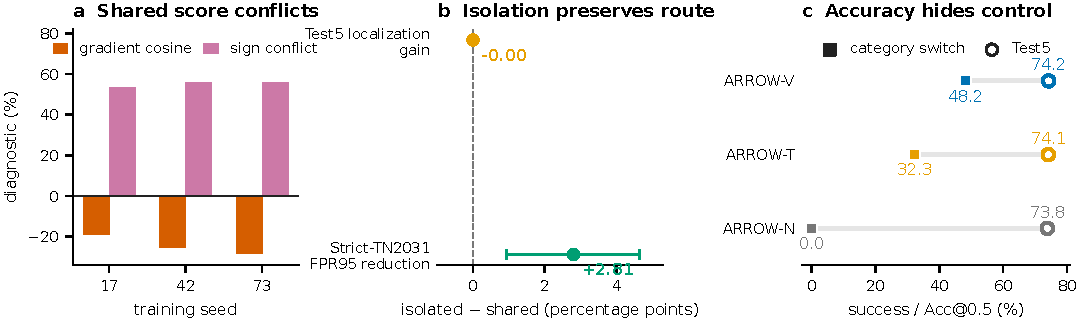
\includegraphics[width=\textwidth]{figures/fig3_mechanism_controllability.pdf}%
  }{\fbox{\parbox[c][1.15in][c]{0.96\textwidth}{\centering
    Gradient conflict, paired ownership effects, and V/T/N category-switch
    controllability generated from registry CSVs.}}}
  \caption{Mechanism evidence.  Shared-duty gradients conflict, structural
  isolation preserves localization while improving rejection, and nearly flat
  standard accuracy hides large differences in category controllability.}
  \label{fig:mechanism}
\end{figure*}

% Generated by paper/scripts/make_main_tables.py.
\begin{table}[t]
\centering
\caption{Admission cues.  FineCops columns use one exact-support matched
surface; the switch panel changes only the named category cue.}
\label{tab:admission}
\scriptsize
\setlength{\tabcolsep}{0.8pt}
\begin{tabular}{lccccc}
\toprule
Cue & Test5$\uparrow$ & Switch$\uparrow$ & P@1$\uparrow$ & Text R@1$\uparrow$ & Image R@1$\uparrow$ \\
\midrule
Visual support & 74.24 $\pm$ 0.09 & 48.24 & 44.16 & 45.05 & 46.14 \\
Category text & 74.12 $\pm$ 0.29 & 32.29 & 43.70 & 44.50 & 45.43 \\
Learned null & 73.83 $\pm$ 0.62 & 0.00 & 42.11 & 42.96 & 43.87 \\
\bottomrule
\end{tabular}
\vspace{2pt}
\parbox{0.98\columnwidth}{\scriptsize Percentages; Test5 is mean $\pm$
sample SD over all three seeds. Visual$-$text switch gain is
+15.95 pp
[$10.81$, $20.83$];
text$-$null is +32.29 pp
[$28.65$, $36.00$]. Visual-support
coverage is 95.60\%; unsupported rows are never counted as rejection.}
\end{table}


\subsection{Endpoint accuracy hides Admission responsibility}
The three capacity-matched cues are close on Test5 but diverge under direct
intervention (Tab.~\ref{tab:admission}, Fig.~\ref{fig:mechanism}).  \arrown
retains 73.83\% Test5 accuracy yet has zero bidirectional category-switch
success.  Canonical text reaches \ArrowTextSwitch\%, and visual support reaches
\ArrowVisualSwitch\%.  The preregistered visual-over-text and text-over-null
confidence intervals both exclude zero.  Matched FineCops results repeat the
ordering on positive P@1 and both negative types.  The supported conclusion is
that visual examples provide category evidence beyond the name, not that
support pixels are required for every correct localization.

% Generated by paper/scripts/make_main_tables.py.
\begin{table}[t]
\centering
\caption{External rejection transfer. FineCops uses standard expression-only
inputs; gRefCOCO is explicitly restricted to single-target/no-target rows.}
\label{tab:external}
\textbf{(a) FineCops-Ref full test}\\[2pt]
\scriptsize
\setlength{\tabcolsep}{1.0pt}
\begin{tabular}{lccccc}
\toprule
Route & P@1$\uparrow$ & T R@1$\uparrow$ & I R@1$\uparrow$ & T AUC$\uparrow$ & I AUC$\uparrow$ \\
\midrule
MM-GDINO-T (published) & 48.45 & 38.69 & 43.14 & 53.98 & 56.52 \\
Original GDINO-T (local) & 44.82 & 41.99 & 41.98 & 54.23 & 53.92 \\
Frozen base & 43.11 & 42.66 & 43.98 & 58.87 & 59.55 \\
Ranking + Abstention & 43.02 & 43.85 & 44.76 & 60.88 & 60.69 \\
\bottomrule
\end{tabular}
\\[5pt]
\textbf{(b) gRefCOCO rejection transfer}\\[2pt]
\scriptsize
\begin{tabular}{llcccc}
\toprule
Slice & Route & AUROC$\uparrow$ & AUPR$\uparrow$ & FPR95$\downarrow$ & Fixed TPR \\
\midrule
Full & Base & 68.95 & 72.01 & 74.10 & -- \\
 & Rejector & 71.75 & 73.81 & 70.83 & 90.10 \\
Rej.-sup.-disj. & Base & 68.69 & 71.92 & 74.97 & -- \\
 & Rejector & 71.50 & 73.73 & 71.16 & 89.72 \\
\bottomrule
\end{tabular}
\\[-1pt]
\parbox{0.98\columnwidth}{\scriptsize T/I denote negative text/image.
The published MM-GDINO-T row is context, not a local or paired comparison.
The local original row loads the unmodified OGC checkpoint with its native
max-token score.  AUC uses the pinned official evaluator's historical
level-1-positive scope for every FineCops row. Fixed TPR uses the sealed source
source threshold; it is never refit. Multi-target gRefCOCO is excluded.}
\end{table}


\subsection{Rejection ordering transfers; the operating point does not}
Table~\ref{tab:external} reports both external surfaces.  On complete
FineCops, the text-cue \arrowt route trails the published
MM-GDINO-T positive P@1 but has numerically higher negative-expression and
negative-image Recall@1.  Because \arrowt receives the structured target noun,
this published row is a reference rather than an input-matched contrast.  We
claim transfer against our same-forward frozen controls, not FineCops SOTA.
\arrowv's support-conditioned result is kept on its matched covered surface and
is never substituted into a full-test row.

On gRefCOCO Full, AUROC rises from 0.6895 to 0.7175 and FPR95 falls from 0.7410
to 0.7083.  On Rejector-supervision-disjoint, AUROC rises from 0.6869 to 0.7150
and FPR95 falls from 0.7497 to 0.7116; all four paired gain intervals exclude
zero.  Because Stage-A saw every image, this controls rejector-supervision
overlap only.  It is evidence about no-target rejection rather than a new
localization domain.

\begin{figure}[t]
  \centering
  \IfFileExists{figures/fig4_external_transfer.pdf}{%
    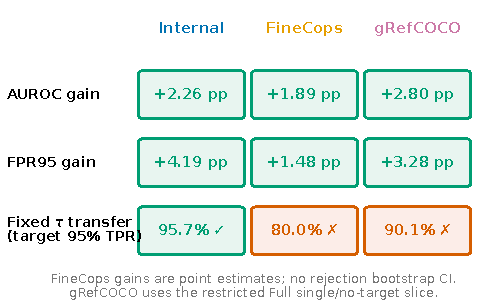
\includegraphics[width=\columnwidth]{figures/fig4_external_transfer.pdf}%
  }{\fbox{\parbox[c][1.05in][c]{0.96\columnwidth}{\centering
    Internal, FineCops, and gRefCOCO rejection ordering versus fixed-threshold
    positive TPR, shown on separate aligned axes.}}}
  \caption{Relative rejection discrimination improves across three negative
  constructions.  The internally sealed threshold reaches its intended source
  operating point but yields only \ArrowFineCopsFixedTPR\% TPR on FineCops and
  \ArrowGrefFixedTPR\% on gRefCOCO.  Thresholds are never fit externally.}
  \label{fig:external}
\end{figure}

Figure~\ref{fig:external} shows that the fixed source threshold under-accepts
external positives.  Improved
AUROC and dataset-normalized FPR95 are compatible with this shift: \method
learns a more transferable positive-versus-negative ordering, while score
offset, scale, and tails remain domain-dependent.  Cross-domain operating-point
calibration is a separate, unresolved problem.
